\documentclass[tikz,border=3pt]{standalone}
\usepackage[utf8]{inputenc}
\usepackage[T1]{fontenc}
\usepackage{lmodern}
\renewcommand{\familydefault}{\sfdefault}
\usepackage{sansmath}\sansmath
\usepackage{chemfig}
\usepackage{pgfplots}\pgfplotsset{compat=1.18,/pgf/number format/use comma,/pgf/number format/1000 sep={.}}
\usetikzlibrary{arrows.meta,calc,positioning,decorations.pathmorphing,patterns}
% paleta del sitio
\definecolor{nar}{HTML}{E8680C}\definecolor{narc}{HTML}{FFB35C}\definecolor{hielo}{HTML}{FFF3E8}
\definecolor{tinta}{HTML}{1D1D1F}\definecolor{gris}{HTML}{6E6E73}\definecolor{lila}{HTML}{7C5CF0}
\definecolor{azul}{HTML}{2F6FD6}\definecolor{menta}{HTML}{17A673}\definecolor{coral}{HTML}{E8342A}
\begin{document}
\newcommand{\amonita}[2]{\begin{scope}[shift={(#1,#2)}]\fill[narc!60] (0,0) circle (0.3);\draw[nar!70!black,thick,domain=0:1080,samples=120,variable=\t] plot ({0.0007*\t^0.85*cos(\t)},{0.0007*\t^0.85*sin(\t)});\end{scope}}
\newcommand{\trilobite}[2]{\begin{scope}[shift={(#1,#2)}]\fill[gris!55] (0,0) ellipse (0.24 and 0.33);\fill[gris!80] (0,0.24) ellipse (0.2 and 0.1);\draw[gris!90!black,thin] (-0.07,-0.3)--(-0.07,0.15) (0.07,-0.3)--(0.07,0.15);\foreach \y in {-0.2,-0.1,0,0.1} \draw[gris!90!black,thin] (-0.2,\y)--(0.2,\y);\end{scope}}
\newcommand{\pez}[2]{\begin{scope}[shift={(#1,#2)}]\fill[azul!45] (0,0) ellipse (0.36 and 0.15);\fill[azul!45] (0.3,0) -- (0.52,0.16) -- (0.52,-0.16) -- cycle;\fill[tinta] (-0.22,0.03) circle (0.025);\draw[azul!70!black,thin] (-0.1,-0.1)--(-0.1,0.1) (0,-0.12)--(0,0.12) (0.1,-0.11)--(0.1,0.11);\end{scope}}
\newcommand{\helecho}[2]{\begin{scope}[shift={(#1,#2)}]\draw[menta!80!black,thick] (0,-0.32)--(0,0.32);\foreach \y/\l in {-0.22/0.2,-0.1/0.18,0.02/0.15,0.14/0.11,0.24/0.07}{\fill[menta!70] (-\l/2-0.02,\y) ellipse ({\l/2} and 0.04);\fill[menta!70] (\l/2+0.02,\y) ellipse ({\l/2} and 0.04);}\end{scope}}
\newcommand{\concha}[2]{\begin{scope}[shift={(#1,#2)}]\fill[lila!35] (0,-0.25) -- (-0.3,0.08) arc (180:0:0.3) -- cycle;\foreach \a in {30,60,90,120,150} \draw[lila!80!black,thin] (0,-0.25) -- ($(0,0.08)+(\a:0.28)$);\end{scope}}

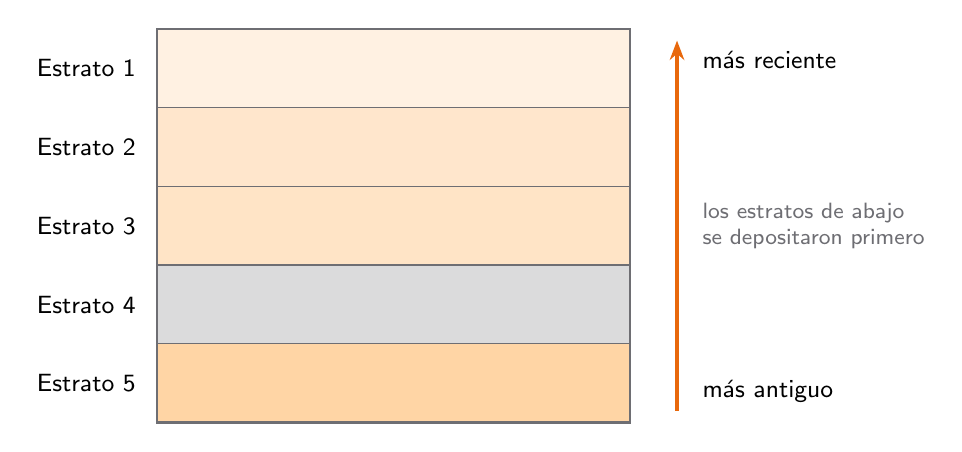
\begin{tikzpicture}[font=\small]
\foreach \y/\c in {0/narc!55,1/gris!25,2/narc!35,3/hielo!80!narc,4/narc!18} \fill[\c] (0,\y) rectangle (6,\y+1);
\foreach \y in {1,2,3,4} \draw[gris,thin] (0,\y) -- (6,\y);
\draw[gris,thick] (0,0) rectangle (6,5);
\foreach \n/\y in {1/4.5,2/3.5,3/2.5,4/1.5,5/0.5} \node[anchor=east] at (-0.15,\y) {Estrato \n};
\trilobite{1.2}{0.5}\trilobite{3.6}{0.5}\trilobite{4.9}{0.45}
\trilobite{1.9}{1.5}\amonita{3.4}{1.5}
\amonita{1.5}{2.5}\amonita{4.4}{2.5}\pez{2.9}{2.5}
\pez{1.6}{3.5}\pez{4.3}{3.5}\helecho{3.1}{3.5}
\helecho{1.2}{4.5}\concha{2.9}{4.5}\concha{4.7}{4.5}
\draw[-{Stealth[length=7pt]},very thick,nar] (6.6,0.15) -- (6.6,4.85);
\node[anchor=west,align=left] at (6.8,4.6) {más reciente};
\node[anchor=west,align=left] at (6.8,0.4) {más antiguo};
\node[anchor=west,align=left,text=gris,font=\footnotesize] at (6.8,2.5) {los estratos de abajo\\se depositaron primero};
\end{tikzpicture}
\end{document}
